%% Thermodynamic feasibility testing of useful-work claims
%% Prepared with the ACS achemso class for Industrial & Engineering Chemistry Research (two-column layout).
%% Build: pdflatex manuscript && bibtex manuscript && pdflatex manuscript && pdflatex manuscript
%% (works unchanged on Overleaf, which includes achemso).
\documentclass[journal=iecred,manuscript=article,layout=twocolumn,email=false]{achemso}

\usepackage[T1]{fontenc}
\usepackage{mathptmx}
\usepackage[scaled=0.92]{helvet}
\usepackage[version=4]{mhchem}
\usepackage{amsmath}
\usepackage{graphicx}
\usepackage{booktabs}
\usepackage{tabularx}
\usepackage{siunitx}
\usepackage{tikz}
\usetikzlibrary{positioning,arrows.meta,shapes.misc}
\usepackage{xurl}
\urlstyle{same}
\sisetup{detect-all, group-digits=integer, group-separator={,}, group-minimum-digits=5}
\setkeys{acs}{articletitle=true}

% CL 202 Group IA (name and roll number)
\author{Madire Sai Preetham (25110183)}
\author{Keshavi Chhodavadia (25110163)}
\author{Sondharva Dimple (25110305)}
\author{Shikha Ajeet Singh (25110292)}
\author{Hrushva Vijaykumar Vadsara (25110332)}
\affiliation[IIT Gandhinagar]{CL 202 Group IA, Department of Chemical Engineering, Indian Institute of Technology
Gandhinagar, Palaj, Gandhinagar 382355, Gujarat, India}

\title{Thermodynamic Feasibility Testing of Useful-Work Claims with a Nine-Model First- and Second-Law Screening Tool}
\abbreviations{COP, coefficient of performance}
\keywords{thermodynamic feasibility, second law, entropy generation, exergy, reversible work}

\begin{document}

\begin{abstract}
Claims about energy-conversion devices are often judged by the First Law alone, although a claim can conserve
energy and still require more work than its source can supply. We developed an open, browser-accessible tool that
screens such claims with the First and Second Laws. The tool assigns each claim to one of nine models: fixed-reservoir
heat engines, finite hot and cold streams, steady control volumes, closed systems, refrigerators and heat pumps,
heat exchangers without shaft work, mechanical harvesters (walking, pedalling, wind and hydro), ideal solar
radiation conversion and electrochemical cells. Each model evaluates its mass, energy and entropy balances together
with the reversible limit that applies to it: the Carnot efficiency or COP, the exact finite-stream limit, the Betz
limit, the Petela--Landsberg radiation exergy or $-\Delta_rG$. The tool then returns a feasible, not feasible or
insufficient-data verdict. A rule-based analyzer reads plain-English problem statements, converts units and selects
the model. Values that the balances fix uniquely are calculated, and missing data are requested rather than assumed.
The models reproduced seven published closed-form results, among them the Bejan--Alebrahim hot-stream exergy and the
Betz and Petela--Landsberg limits, to within \SI{0.001}{\percent}. They matched published data for liquid water and
the hydrogen fuel cell to within \SI{0.05}{\percent}, and a measured harvester output lay below the computed ceiling as
required. A refrigerator exergy efficiency differed by \SI{9.5}{\percent} from a published simulation because the
evaporating temperature is defined differently. Of 63 independently written test scenarios, 56 matched the
expected verdict. The remaining seven were justified by the added refrigeration model or by incomplete data.
\end{abstract}

% =============================================================================================
\section{Introduction}
% =============================================================================================
Energy-conversion proposals, from waste-heat engines to wearable harvesters, are frequently presented with a claimed
power output or efficiency. Conservation of energy is necessary but not sufficient for such a claim to be possible.
The Second Law restricts which energy can be converted into work, and the limit depends on the temperatures, streams
or chemical potentials that the device actually has access to. Historically, Carnot's analysis of heat engines was the
first statement of this restriction. Clausius and Thomson then generalized it to the entropy principle, and later work
recast it as the theory of exergy, the maximum useful work obtainable as a system comes to equilibrium with its
environment.\cite{Wang2017} Xue and Guo returned to Clausius' own writings and showed that he regarded the equivalence of
transformations, rather than the familiar sentence that heat cannot pass unaided from a colder to a warmer body, as the
statement of the Second Law. From it they derived a general relation among the heat, the work and the temperatures of
an arbitrary cycle.\cite{Xue2019} Lee et al.\ derived the Clausius inequality from the First Law and thermodynamic
stability conditions alone, without the Carnot cycle and without either classical statement.\cite{Lee2014} Both papers
support the viewpoint a feasibility test needs: the Second Law is a quantitative inequality that applies to any device.
A claim is rejected when the entropy it implies is negative, whatever device is proposed.

Exergy analysis turns these principles into engineering numbers. Demirel reviewed second-law, exergy, pinch and related analyses. He found exergy
analysis to be the most widely used, applied to power cycles, solar energy, refrigeration and waste-heat utilization,
and identified the assessment of thermodynamic imperfections as its common aim.\cite{Demirel2013} The Gouy--Stodola theorem links the two quantities directly: the work lost in a process
equals $T_0\dot S_\mathrm{gen}$. Pal examined the conditions under
which the theorem applies to open systems and noted that the lost work is a relative quantity, which depends on the
chosen environment temperature.\cite{Pal2017} He also showed how entropy generation in a
familiar process, viscous flow through packed beds, makes the Second Law concrete for chemical engineering
students.\cite{Pal2019} Mady et al.\ applied the same exergy efficiency to household refrigerators, heat pumps and
water heaters. They showed that a COP alone can mislead, because the Carnot limit itself changes with the operating
temperatures.\cite{Mady2020}

A practical difficulty remains: the correct limit depends on the physical situation. A heat engine between two
reservoirs is bounded by the Carnot efficiency. An engine driven by a hot stream that cools as it gives up heat has a
lower limit. Bejan and Alebrahim showed that this limit is set by the stream exergy and by the heat-capacity rate of
the cold side.\cite{Bejan2001} Wind, hydro and walking harvesters are bounded by their mechanical resource
instead,\cite{Betz1920,Li2009} solar converters by the exergy of radiation,\cite{Petela2003} and fuel cells by the
Gibbs energy of reaction.\cite{NETL2004} Applying the Carnot expression to every claim is therefore wrong in both
directions: it can accept impossible claims and reject possible ones.

This work presents the Thermodynamic Feasibility Tester, a screening tool that (i) maps a described claim onto a
system boundary and one of nine models, (ii) evaluates the mass, energy and entropy balances that the data allow, and
(iii) compares the claim with the model's reversible or resource limit. The tool returns one of three outcomes:
feasible within the stated model, not feasible, or insufficient data. The last outcome stops the tool from inventing
values, which is a common source of error when users or language models fill in a gap. The tool runs in a web browser
as well as from a terminal. All calculations are deterministic Python and every result shows its equations. We
describe the models, validate them against literature and analytical data, and verify the complete workflow against
63 independently written test scenarios.

% =============================================================================================
\section{Theory and Methodology}
% =============================================================================================
\subsection{Feasibility criteria}
A claim is tested on a stated boundary. It is rejected if any applicable balance fails: mass ($\sum\dot m_\mathrm{in}
=\sum\dot m_\mathrm{out}$ at steady state), energy, or entropy, where entropy generation must satisfy
$\dot S_\mathrm{gen}\ge0$.\cite{Wang2017,Xue2019} It is also rejected if the claimed useful output exceeds the model's
reversible or resource limit. If every applicable check passes, the verdict is \emph{feasible / not rejected}, which
means only that the claim is thermodynamically admissible for the stated model. If a required value is missing, the
verdict is \emph{insufficient data} and the missing quantity is named. Values that a balance fixes uniquely are
calculated rather than requested, for example a stream outlet temperature, the rejected heat $\dot Q_C=\dot Q_H-\dot W$,
or the third of $\dot Q_C$, $\dot Q_H$ and $\dot W_\mathrm{in}$.

\subsection{Thermal models}
\textbf{Model 1, fixed-temperature reservoirs.} For a cyclic engine with heat magnitudes $\dot Q_H$ and $\dot Q_C$,
\begin{gather}
\dot Q_H=\dot W+\dot Q_C,\qquad
\dot S_\mathrm{gen}=\frac{\dot Q_C}{T_C}-\frac{\dot Q_H}{T_H}\ge0,\nonumber\\
\eta=\frac{\dot W}{\dot Q_H}\le1-\frac{T_C}{T_H}.
\label{eq:carnot}
\end{gather}

\textbf{Model 2, finite hot and cold streams.} A hot stream ($\dot m_h$, $c_{p,h}$) cooled from $T_{h,1}$ to $T_{h,2}$
releases $\dot Q_h=\dot m_h\int c_{p,h}\,\mathrm{d}T$ to a cyclic device that rejects heat to a cold stream entering at
$T_{c,1}$. The exact limit is found by setting $\dot S_\mathrm{gen}=0$ for the complete boundary. This gives the
reversible cold outlet $T_{c,\mathrm{rev}}$, which for constant heat capacities is
\begin{gather}
T_{c,\mathrm{rev}}=T_{c,1}\left(\frac{T_{h,1}}{T_{h,2}}\right)^{\dot m_hc_{p,h}/(\dot m_cc_{p,c})},\nonumber\\
\dot W_\mathrm{max}=\dot Q_h-\dot m_cc_{p,c}\left(T_{c,\mathrm{rev}}-T_{c,1}\right).
\label{eq:finite}
\end{gather}
As $\dot m_cc_{p,c}\to\infty$, eq~\ref{eq:finite} tends to the stream exergy
$\dot m_hc_{p,h}[(T_{h,1}-T_0)-T_0\ln(T_{h,1}/T_0)]$ of Bejan and Alebrahim.\cite{Bejan2001} A claim is tested against
$\dot W_\mathrm{max}$. If no work is claimed, the limit is reported alone.

\textbf{Model 3, steady control volume.} For turbines, compressors, pumps and nozzles,
\begin{align}
0&=\dot Q-\dot W+\textstyle\sum_\mathrm{in}\dot m\,\theta-\sum_\mathrm{out}\dot m\,\theta,\\
\dot S_\mathrm{gen}&=\textstyle\sum_\mathrm{out}\dot ms-\sum_\mathrm{in}\dot ms-\sum_j\dot Q_j/T_{b,j}\ge0.
\end{align}
where $\theta=h+V^2/2+gz$ is the specific energy of each stream.

\textbf{Model 4, closed system.} $Q-W=\Delta E$ and $S_\mathrm{gen}=\Delta S-\sum_jQ_j/T_{b,j}\ge0$. A complete cycle has
$\Delta E=\Delta S=0$. Each balance is evaluated only when its data are present, so an energy imbalance alone is enough
to reject a claim.

\textbf{Model 5, refrigerator or heat pump.} With work input $\dot W_\mathrm{in}$, $\dot Q_H=\dot Q_C+\dot W_\mathrm{in}$,
$\dot S_\mathrm{gen}=\dot Q_H/T_H-\dot Q_C/T_C$, and
\begin{gather}
\mathrm{COP}_R=\frac{\dot Q_C}{\dot W_\mathrm{in}}\le\frac{T_C}{T_H-T_C},\nonumber\\
\mathrm{COP}_{HP}=\frac{\dot Q_H}{\dot W_\mathrm{in}}\le\frac{T_H}{T_H-T_C}.
\end{gather}
The second-law (exergy) efficiency of Mady et al.\ is $\mathrm{COP}/\mathrm{COP}_\mathrm{Carnot}$.\cite{Mady2020}

\textbf{Model 6, heat exchanger.} With no shaft work, $\dot Q_h=\dot Q_c$ for an insulated unit (within
\SI{0.1}{\percent}, to allow rounded data), or $\dot Q_h=\dot Q_c+\dot Q_\mathrm{loss}$ when a loss is stated. The checks
are $\dot S_\mathrm{gen}=\sum\dot m\int c_p\,\mathrm{d}T/T\ge0$ and the absence of a temperature cross
($T_{c,\mathrm{out}}\le T_{h,\mathrm{in}}$ and $T_{h,\mathrm{out}}\ge T_{c,\mathrm{in}}$ in counterflow). The exergy
destroyed, $T_0\dot S_\mathrm{gen}$, is reported when $T_0$ is given.\cite{Pal2017}

\subsection{Resource-limited models}
\textbf{Model 7, mechanical harvesting.} The electrical output cannot exceed the recoverable mechanical input:
$E_\mathrm{step}f$ or $F\,d\,f$ for walking, $\tau\omega$ for pedalling, $\rho gQH$ for hydro, and
$\tfrac{16}{27}\cdot\tfrac12\rho Av^3$ for wind (the Betz limit).\cite{Betz1920} A claim with no input is rejected.

\textbf{Model 8, solar radiation.} For undiluted blackbody radiation at $T_s$ received by area $A$ at irradiance $G$,
the ideal work ceiling is\cite{Petela2003}
\begin{equation}
\dot W_\mathrm{max}=GA\left[1-\frac43\frac{T_0}{T_s}+\frac13\left(\frac{T_0}{T_s}\right)^4\right].
\label{eq:petela}
\end{equation}

\textbf{Model 9, electrochemical conversion.} At constant $T$ and $p$, the maximum non-expansion work is
$-\Delta_rG$ per mole of reaction, so $\dot W_\mathrm{max}=-\Delta_rG\,\dot\xi$. A positive $\Delta_rG$ gives no
work.\cite{NETL2004}

\textbf{Property utility and fallback.} Two non-numbered helpers support the models. The first calculates $\Delta h=\int
c_p\,\mathrm{d}T$ and $\Delta s=\int c_p\,\mathrm{d}T/T$ (constant or linear $c_p$), latent contributions $L$ and $L/T$,
and the effective temperature $\Delta h/\Delta s$. The second returns \emph{model required} for processes with no
validated model, such as transient conduction or tidal energy, instead of forcing an unrelated model.

% =============================================================================================
\section{Computational Details}
% =============================================================================================
\begin{figure}
\centering
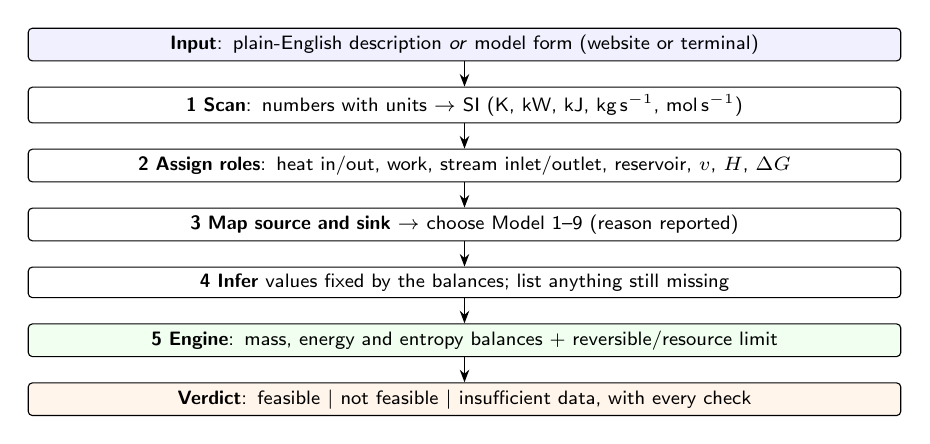
\begin{tikzpicture}[node distance=3.2mm, font=\sffamily\scriptsize,
  box/.style={draw, rounded corners=1.5pt, align=center, text width=0.9\columnwidth, inner sep=2.4pt, fill=#1},
  box/.default=white, arr/.style={-{Stealth[length=1.6mm]}, semithick}]
\node[box=blue!6] (a) {\textbf{Input}: plain-English description \emph{or} model form (website or terminal)};
\node[box, below=of a] (b) {\textbf{1 Scan}: numbers with units $\rightarrow$ SI (K, kW, kJ, kg\,s$^{-1}$, mol\,s$^{-1}$)};
\node[box, below=of b] (c) {\textbf{2 Assign roles}: heat in/out, work, stream inlet/outlet, reservoir, $v$, $H$, $\Delta G$};
\node[box, below=of c] (d) {\textbf{3 Map source and sink} $\rightarrow$ choose Model 1--9 (reason reported)};
\node[box, below=of d] (e) {\textbf{4 Infer} values fixed by the balances; list anything still missing};
\node[box=green!6, below=of e] (f) {\textbf{5 Engine}: mass, energy and entropy balances + reversible/resource limit};
\node[box=orange!8, below=of f] (g) {\textbf{Verdict}: feasible $\mid$ not feasible $\mid$ insufficient data, with every check};
\foreach \x/\y in {a/b,b/c,c/d,d/e,e/f,f/g} \draw[arr] (\x) -- (\y);
\end{tikzpicture}
\caption{Workflow of the tester. Steps 1--4 belong to the analyzer and are used only for written descriptions. The
engine (step 5) is identical for the website, the terminal program and saved JSON cases.}
\label{fig:workflow}
\end{figure}

The tool is written in Python~3 using only the standard library (Figure~\ref{fig:workflow}). The calculation engine
(\num{1774} lines) contains the nine models, the property utility, the balances and a common verdict routine. It
can be run from the terminal, on saved JSON cases, or through the website. Heat capacities are integrated analytically
for constant and linear $c_p$. Balances are tested against an absolute tolerance of $10^{-8}$ plus a relative
tolerance of $10^{-6}$ of the largest term. Resource ceilings are tested with a relative tolerance of $10^{-9}$, so a
claim exactly at the limit is accepted as the reversible case. Every result carries a table of checks giving the
check, the equation, the calculated value, the criterion and PASS, FAIL, NOT EVALUATED or NOT APPLICABLE.

The analyzer (\num{2306} lines) reads a plain-English description. It recognizes numbers with their units (including
\si{\degreeCelsius}, $^\circ$F, Btu\,h$^{-1}$, L\,min$^{-1}$, rpm and number words) and assigns each
quantity a role from the surrounding words. It then groups hot and cold streams separately from fixed-temperature
reservoirs and chooses the model, reporting the words that pointed to it. Defaults, such as $c_p$ of water or an air
density, are used only when the text names the substance, and each default is listed in the result. Energy amounts and
rates are never mixed.

The website (\url{https://keshavichhodavadia-del.github.io/thermodynamic-feasibility-tester/}; source code at
\url{https://github.com/keshavichhodavadia-del/thermodynamic-feasibility-tester}) runs the same Python
engine in the visitor's browser through Pyodide in a web worker, so no server or API key is needed. The site offers a
form for each model and a description box. It provides 43 worked examples in eight categories, nine homepage examples
(one per model), and charts drawn from the engine's results (energy path, First-Law closure, entropy-generation gauge,
temperature profile). A sensitivity sweep re-runs a model while one input varies. Verification uses 83 Python unit
tests, which include all 63 scenarios of the team's test-case document, 10 website tests and a 27-case engine
self-test. Every figure and data file in this work is regenerated by scripts in the code package.

% =============================================================================================
\section{Results and Discussion}
% =============================================================================================
\subsection{Validation against literature data}
Table~\ref{tbl:validation} and Figure~\ref{fig:validation} compare the models with the literature in two ways. Part
(a) compares results with numbers reported in the literature: property tables, a fuel-cell handbook, a published
refrigeration simulation and a measured harvester. Part (b) checks each model against a closed-form result published
for the same situation. The reference value is computed independently of the engine, so part (b) confirms that the
published equations are implemented correctly, while part (a) tests the models against independent data. All seven
closed-form checks agree to better than \SI{0.001}{\percent}, and six are exact to machine precision. Model 1
reproduces the Carnot efficiency. Model 3 reproduces $\dot S_\mathrm{gen}=\dot m(s_2-s_1)=\SI{0.6}{\kilo\watt\per\kelvin}$ for an adiabatic
turbine, which corresponds to a Gouy--Stodola lost work of \SI{179}{\kilo\watt} at \SI{298.15}{\kelvin},\cite{Pal2017}
and Model 6 reproduces the entropy generated in a water--water exchanger. For Model 4, moving \SI{100}{\kilo\joule} from
\SI{300}{\kelvin} to \SI{600}{\kelvin} with no work gives $S_\mathrm{gen}=-\SI{0.1667}{\kilo\joule\per\kelvin}$ and a
\emph{not feasible} verdict, as the Clausius statement requires.\cite{Xue2019} Models 7 and 8 reproduce the Betz
limit\cite{Betz1920} and eq~\ref{eq:petela} for $T_s=\SI{6000}{\kelvin}$ and $T_0=\SI{300}{\kelvin}$.\cite{Petela2003}

\begin{table*}
\caption{Validation of the Models against the Literature: (a) Published Data, (b) Published Closed-Form Results}
\label{tbl:validation}
\footnotesize
\setlength{\tabcolsep}{4pt}
\begin{tabular}{@{}l l l S[table-format=4.4] S[table-format=4.4] S[table-format=-1.5] l@{}}
\toprule
model & quantity & conditions & {reference} & {code} & {difference (\%)} & reference basis \\
\midrule
\multicolumn{7}{@{}l}{\textit{(a) Comparison with published data}} \\
5 & exergy efficiency (\%) & 3/25\,\si{\degreeCelsius}, COP 3.1 & 27.3 & 24.70 & -9.5 & R410A simulation\cite{Mady2020} \\
7 & harvester output (W) & generative braking & 2.4 & 4.4 & {--} & measured $\le$ ceiling\cite{Li2009} \\
9 & fuel-cell ceiling (kW) & \ce{H2}, 0.01\,mol/s & 2.37161 & 2.37141 & -0.0084 & $nFE$, 1.229\,V\cite{NETL2004} \\
-- & $\Delta h$ of water (kJ/kg) & 298.15$\to$340\,K, 1\,bar & 175.018 & 175.100 & 0.047 & JANAF table\cite{Chase1998} \\
\midrule
\multicolumn{7}{@{}l}{\textit{(b) Check against published closed-form results}} \\
1 & Carnot efficiency (\%) & 600/300\,K & 50.0 & 50.0 & 0 & Carnot\cite{Wang2017} \\
2 & $\dot W_\mathrm{max}$ (kW) & water, 90$\to$25\,\si{\degreeCelsius} & 25.9121 & 25.9119 & -0.00094 & stream exergy\cite{Bejan2001} \\
3 & $\dot S_\mathrm{gen}$ (kW/K) & turbine, $s_1=6.8$, $s_2=7.1$ & 0.6 & 0.6 & 0 & $\dot m(s_2-s_1)$\cite{Pal2017} \\
4 & $S_\mathrm{gen}$ (kJ/K) & \SI{100}{kJ}, 300$\to$600\,K & -0.1667 & -0.1667 & 0 & Clausius\cite{Xue2019} \\
6 & $\dot S_\mathrm{gen}$ (kW/K) & water--water exchanger & 0.028385 & 0.028385 & 0 & $\sum\dot mc_p\ln(T_2/T_1)$\cite{Pal2019} \\
7 & Betz ceiling (W) & $A=10$\,m$^2$, $v=8$\,m/s & 1858.37 & 1858.37 & 0 & Betz\cite{Betz1920} \\
8 & radiation ceiling (kW) & $GA=2$\,kW, $T_s=6000$\,K & 1.86667 & 1.86667 & 0 & eq~\ref{eq:petela}\cite{Petela2003} \\
\bottomrule
\end{tabular}
\end{table*}

\begin{figure}
\centering
\includegraphics[width=\columnwidth]{figures/fig2_validation.pdf}
\caption{Relative difference between the code and the reference for each validation case of
Table~\ref{tbl:validation}. Bars marked ``exact'' agree to machine precision. The dotted line marks \SI{1}{\percent}.}
\label{fig:validation}
\end{figure}

The small differences have clear causes. The \SI{0.00094}{\percent} difference for Model 2 comes from using a
finite cold stream (\SI{e5}{kg/s}) to represent the environment. Figure~\ref{fig:maps}d shows $\dot W_\mathrm{max}$ rising
monotonically toward the Bejan--Alebrahim exergy as the cold stream grows.\cite{Bejan2001} When the hot stream is cooled
all the way to $T_0$, a cold stream no larger than the hot one leaves no work to extract: the reversible cold outlet
then reaches the hot inlet temperature. This illustrates why a fixed-reservoir Carnot estimate overstates the
finite-stream limit. For Model 9, the \SI{0.0084}{\percent} difference reflects the rounded \SI{1.229}{\volt}
reversible voltage compared with the JANAF Gibbs energy of \SI{-237.141}{\kilo\joule\per\mole},\cite{NETL2004,Chase1998}
and the \SI{0.047}{\percent} error of the property utility is the constant-$c_p$ approximation for liquid
water.\cite{Chase1998}

The largest difference is for Model 5. Mady et al.\ simulated an R410A vapour-compression cycle evaporating at
\SI{3}{\degreeCelsius} with surroundings at \SI{25}{\degreeCelsius}. They reported a COP of 3.1 and an exergy efficiency
of \SI{27.3}{\percent}.\cite{Mady2020} Their eq 14 applied to the stated temperatures gives \SI{24.7}{\percent}, the same
value as the tool, so the \SI{9.5}{\percent} difference is not an error in the COP limit. It is consistent with a
refrigerant evaporating near \SI{0.9}{\degreeCelsius}, about \SI{2}{\kelvin} below the stated evaporator temperature. The
published simulation does not report enough states to confirm this. The comparison shows how strongly the Carnot COP,
and therefore any COP claim, depends on the temperatures used: a \SI{2}{\kelvin} change moves the limit by about
\SI{10}{\percent}.

For the mechanical model (Table~\ref{tbl:validation}a), the knee-mounted harvester of Li et al.\ supplied \SI{4.4}{\watt} of mechanical power in
generative-braking mode and produced \SI{2.4}{\watt} of electricity.\cite{Li2009} The tool places the ceiling at
\SI{4.4}{\watt} and returns \emph{feasible}, with the measured output \SI{45}{\percent} below the ceiling. This is the expected
relation between a resource limit and real device efficiency, \SI{54.6}{\percent} in that study.

\subsection{Feasibility maps}
Figure~\ref{fig:maps} places every evaluated case against its model limit. Heat-engine claims fall on or below
the Carnot line $1-T_C/T_H$ unless they are rejected, and the case exactly on the line is accepted as reversible with
$\dot S_\mathrm{gen}=0$ (panel a). Every feasible refrigerator and heat pump lies below COP $=$ COP$_\mathrm{Carnot}$,
and the three rejected claims lie above it, including a freezer claiming COP 8 where 5.93 is the limit (panel b). The
resource-limited claims of Models 2, 7, 8 and 9 span seven orders of magnitude, from a \SI{5}{\watt} walking generator
to a \SI{5}{\mega\watt} hydro plant, yet all collapse onto one rule: claims above the diagonal are rejected (panel c).
Examples are a \SI{40}{\metre} wind rotor claiming \SI{800}{\kilo\watt} against a Betz ceiling of
\SI{456}{\kilo\watt}, and a methanol cell claiming \SI{0.8}{\kilo\watt} against
$-\Delta_rG\,\dot\xi=\SI{0.70}{\kilo\watt}$.

\begin{figure*}
\centering
\includegraphics[width=\textwidth]{figures/fig3_feasibility_maps.pdf}
\caption{Feasibility maps from the engine's results for all website examples and test scenarios. (a) Model 1 efficiency
against the Carnot limit. (b) Model 5 claimed COP against the Carnot COP (refrigerators and heat pumps). (c) Claimed
output against the model ceiling for Models 2, 7, 8 and 9 (green feasible, red not feasible). (d) Model 2 maximum work
for water cooled from 90 to \SI{25}{\degreeCelsius} as the cold stream (inlet \SI{25}{\degreeCelsius}) grows,
approaching the hot-stream exergy of Bejan and Alebrahim. Shaded regions violate the Second Law.}
\label{fig:maps}
\end{figure*}

\subsection{Verification against independent test scenarios}
The complete workflow, from description to analyzer to engine to verdict, was run on 63 scenarios written
independently by the team. They are grouped in ten sections covering normal claims, infeasible claims, reversible
limits, missing data and out-of-scope processes (Figure~\ref{fig:verification}). In 56 cases the verdict matched the
expected one. The seven differences (Table~\ref{tbl:differences}) are deliberate. In one case the document's expectation was
wrong; two processes became supported when the refrigeration model was added; two cases supplied too little data for
the Second Law; and two depended on an earlier question, which the stateless tool does not remember. In the remaining cases with missing data, the tool named the missing quantity: a reservoir temperature, a cold-stream
inlet, an outlet state, a heat capacity, a rotor area or a reaction rate. A temperature of \SI{-400}{\degreeCelsius} was
rejected as below absolute zero.

\begin{figure}
\centering
\includegraphics[width=\columnwidth]{figures/fig4_verification.pdf}
\caption{Verdicts for the 63 test scenarios by section of the test-case document. Sections: 1 Carnot engines;
2 finite streams; 3 steady flow; 4 closed systems; 5 property changes; 6 out-of-scope and refrigeration; 7 heat
exchangers; 8 mechanical; 9 solar; 10 electrochemical.}
\label{fig:verification}
\end{figure}

\begin{table}
\caption{Test Scenarios Whose Verdict Differs from the Test-Case Document}
\label{tbl:differences}
\scriptsize
\begin{tabularx}{\columnwidth}{@{}l l X@{}}
\toprule
case & tool verdict & reason \\
\midrule
2.1 & not feasible & \SI{20}{kW} claimed exceeds $\dot W_\mathrm{max}=\SI{15.06}{kW}$; the document expected feasible \\
4.4 & insufficient data & no $\Delta S$: First Law only, $U_2=\SI{540}{kJ}$ reported \\
6.1, 6.2 & feasible & refrigerator and heat pump now evaluated by Model 5 (COP 3.33 and 3.5) \\
7.4 & insufficient data & duties only: energy closes, $\dot S_\mathrm{gen}$ needs temperatures \\
8.6, 8.8 & needs data & ``same conditions'' refers to a previous case \\
\bottomrule
\end{tabularx}
\end{table}

\subsection{Scope and limitations}
A \emph{feasible} verdict means only that the claim passes the checks of the stated model. It does not establish that
the device can be built, will be economical or will operate stably. The property models assume constant or linear heat
capacity, so steam and refrigerant states must be supplied from tables. The resource models (7--9) bound the output by
the stated resource and do not resolve internal losses. Model 8 assumes undiluted blackbody radiation. Model 9 requires
$\Delta_rG$ at the operating state. The analyzer is rule-based: unusual phrasing may need the model form, and it does
not carry information between separate questions. Transient conduction and tidal energy return \emph{model required}
rather than an unvalidated estimate.

% =============================================================================================
\section{Conclusions}
% =============================================================================================
A nine-model feasibility tester was developed that applies the First and Second Laws together with the reversible
limit appropriate to each energy source. The limits used are the Carnot efficiency and COP, the exact finite-stream
limit, steady-flow and closed-system entropy balances, the Betz limit, the Petela--Landsberg radiation exergy and
$-\Delta_rG$. The models reproduced seven published closed-form results to within \SI{0.001}{\percent} and
published data for liquid water and the hydrogen fuel cell to within \SI{0.05}{\percent}, and a measured harvester
output lay below its computed ceiling. A refrigerator exergy efficiency differed by \SI{9.5}{\percent} from a
published simulation because of how the evaporating temperature was defined, which shows how sensitive COP limits are
to the stated temperatures. The complete
workflow reproduced 56 of 63 independent test verdicts, and the other seven differences were justified. Separating
model selection from deterministic calculation, and reporting \emph{insufficient data} instead of assuming values,
makes each verdict traceable to stated equations and inputs. The tool is freely usable in a web browser.
Useful extensions are real-fluid property tables for steam and refrigerants, multi-stream control volumes in the web
form, and uncertainty propagation for measured inputs.

\begin{acknowledgement}
The authors thank the CL 202 (Chemical Engineering Thermodynamics) instructors for the project framework.
\end{acknowledgement}

\begin{suppinfo}
The code package (engine, analyzer, website, tests and the scripts that regenerate every figure and data file) and the
input/output data for all 43 website examples and 63 test scenarios, one CSV file and one results file per model,
accompany this manuscript. The website is available at
\url{https://keshavichhodavadia-del.github.io/thermodynamic-feasibility-tester/} and the source code at
\url{https://github.com/keshavichhodavadia-del/thermodynamic-feasibility-tester}.
\end{suppinfo}

\bibliography{references}

\end{document}
